With both anchors in place we swept seeded two-player $3\times3$ families of
exact target $\alpha$ (mixed from unit-norm potential and harmonic components)
and read every meter. Three findings follow, in the order discovered. All are
rank-order statements at fixed $\lambda=1.2$ on this family class unless noted;
per-cell significance is neither claimed nor needed --- surfaces and
within-level correlations carry the content, with bootstrap intervals in the
artifacts.

\subsection{Finding 1: co-movement along $\alpha$, with a marginal--conditional trap}
Marginally, the meters co-move almost perfectly: Spearman
$\rho(\R,\alpha)=0.982$ ($n{=}2000$), $\rho(\EPR,\alpha)=0.990$ and
$\rho(\EPR,\R)=0.993$ ($n{=}1000$). The last number is a trap: stratified by
$\alpha$, the within-level coupling $\rho(\EPR,\R\mid\alpha)$ is $+0.80$ to
$+0.88$ for $\alpha\le0.65$, degrades through $+0.61$ ($\alpha{=}0.75$) and
$+0.32$ ($\alpha{=}0.85$), and \emph{reverses} to $-0.36$ at $\alpha=0.95$.
The marginal 0.993 is $\alpha$-driven confounding. (This stratification was
demanded by the project's adversarial reviewer; the marginal number alone had
survived our own first write-up.)

\subsection{Finding 2: the wedge, and criticality escape}
The $(\lambda,\alpha)$ surface of $\rho(SB)$ shows two regimes
(Fig.~\ref{fig:phase}). On potential games, $\rho$ is \emph{non-monotone} in
$\lambda$: it rises to $\approx0.5$ near $\lambda\approx1.7$ and then collapses
to zero, because the high-$\lambda$ principal branch concentrates on a strict
equilibrium and $C\to0$ exponentially --- $S=\lambda C\to0$ despite the
$\lambda$ factor. Potential games \emph{escape} criticality through equilibrium
concentration. At $\alpha=1$, mixed equilibria keep $C$ bounded away from zero
and $\rho$ grows without bound. In between, a supercritical wedge opens: the
median game first crosses $\rho=1$ at $\alpha=0.5$ ($\lambda\ge8.5$); a 0.2
fraction of individual games crosses already at $\alpha=0.4$; the frontier
descends to $\lambda_c\approx3$ by $\alpha=0.8$. Inside the wedge the resolvent
is near-singular and $\R$ magnitudes are direction-only --- the surface
artifact carries this caveat cell-by-cell.

\subsection{Finding 3: the response and dissipation layers are distinct
(a refuted repair, reported plainly)}
To explain Finding~1 we hypothesised that $\R$'s denominator
$\|\chieq+\chieq{}^\top\|_F$ underflows at high $\alpha$ (the ratio measuring
the residual symmetric sliver), and that the \emph{numerator}
$\|\chieq-\chieq{}^\top\|_F$ would remain a valid circulation gauge. We tested
both on the identical seeded games (paired design). Half held:
$\rho(\R,\,1/\text{den}\mid\alpha)$ climbs monotonically to $0.993$ at
$\alpha=0.95$ --- at high $\alpha$, $\R$'s within-level variation \emph{is} the
shrinking symmetric response. But the repair failed: the numerator also
decouples, $\rho(\text{num},\EPR\mid\alpha{=}0.95)=-0.37$ (95\% bootstrap CI
excluding zero), against $+0.77$ to $+0.86$ for $\alpha\le0.65$. No
renormalisation of the response matrix recovers the dissipation ordering in the
near-harmonic regime.

Our reading --- argued, not proved --- is that $\chieq$ is a local derivative
at the QRE point (a marginal-strategy object) while $\EPR$ is a functional of
the joint-profile stationary flux; nothing identifies one with the other except
in potential games, where both vanish. The practical scope table this yields:
$\R$ answers \emph{``is this system potential?''} exactly, at every $\lambda$
and every $\alpha$; $\EPR$ answers \emph{``how hard is it circulating?''};
$\R$ \emph{levels} are comparable across systems only for $\alpha\lesssim0.65$
(measured at $\lambda=1.2$, $3\times3$, two players; the crossover's $\lambda$-
and size-dependence is open). The refuted hypothesis, its post-hoc origin, and
the sequence of events are recorded in the project's findings log; the gate
protecting this result was specified after measurement as a regression
contract, and says so on its face.

\begin{figure}[t]
\centering
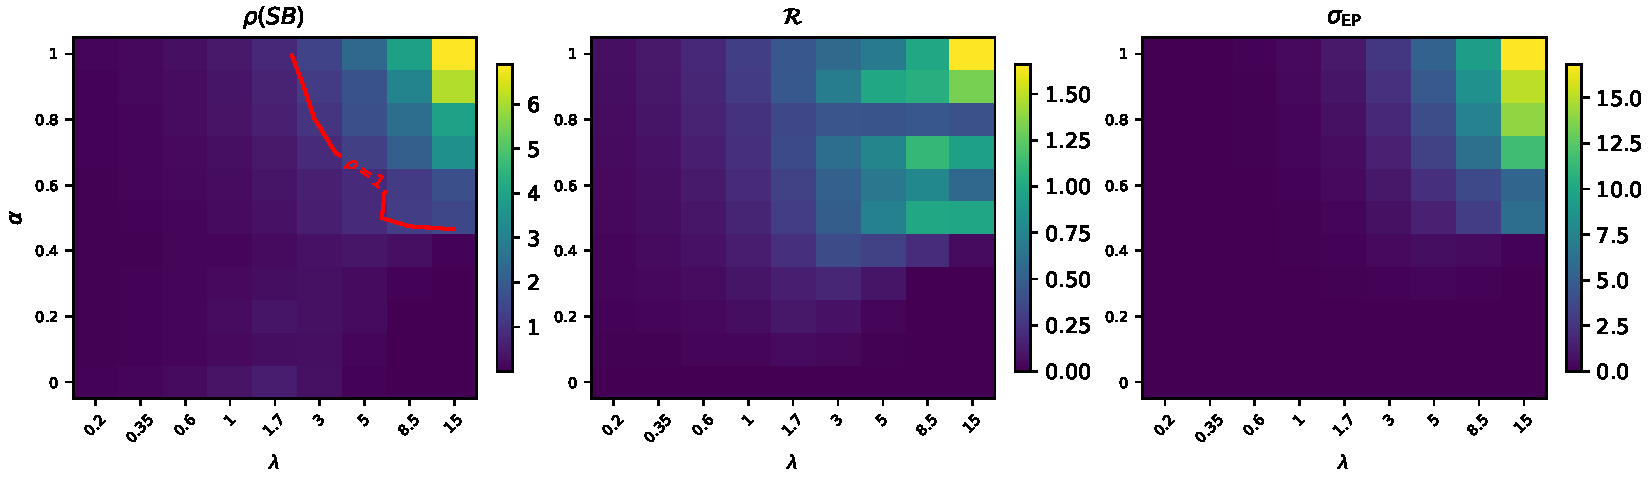
\includegraphics[width=\textwidth]{figures/phase_map.pdf}
\caption{The $(\lambda,\alpha)$ surface: median $\rho(SB)$, $\R$, and $\EPR$
over seeded families (5 games/cell; $\alpha$ increases upward, $\lambda$
rightward). The criticality escape at $\alpha=0$ and the supercritical wedge
are visible in the left panel. Regenerates from
\texttt{experiments/phase\_map.py}, seed 20260808.}
\label{fig:phase}
\end{figure}
